\section{Kerberos Delegation}
\ref{kerberos:delegation}

\subsection{Unconstrained Delegation}

The \verb+UAC+ of the account as the \verb+TRUSTED_FOR_DELEGATION+ flag set (requiere \verb+SeEnableDelegationPrivilege+ to set). The user account to relay must have the \verb+UAC+ \verb+NOT_DELEGATED+ flag unset.

If both prerequisites are met, then the Domain Controller will respond to the user with a \verb+KRB_TGS_REP+ containing standard information, but it will also contains a {\bf copy of the user’s TGT} in his response, and a new associated session key.

\begin{figure}[!ht]
  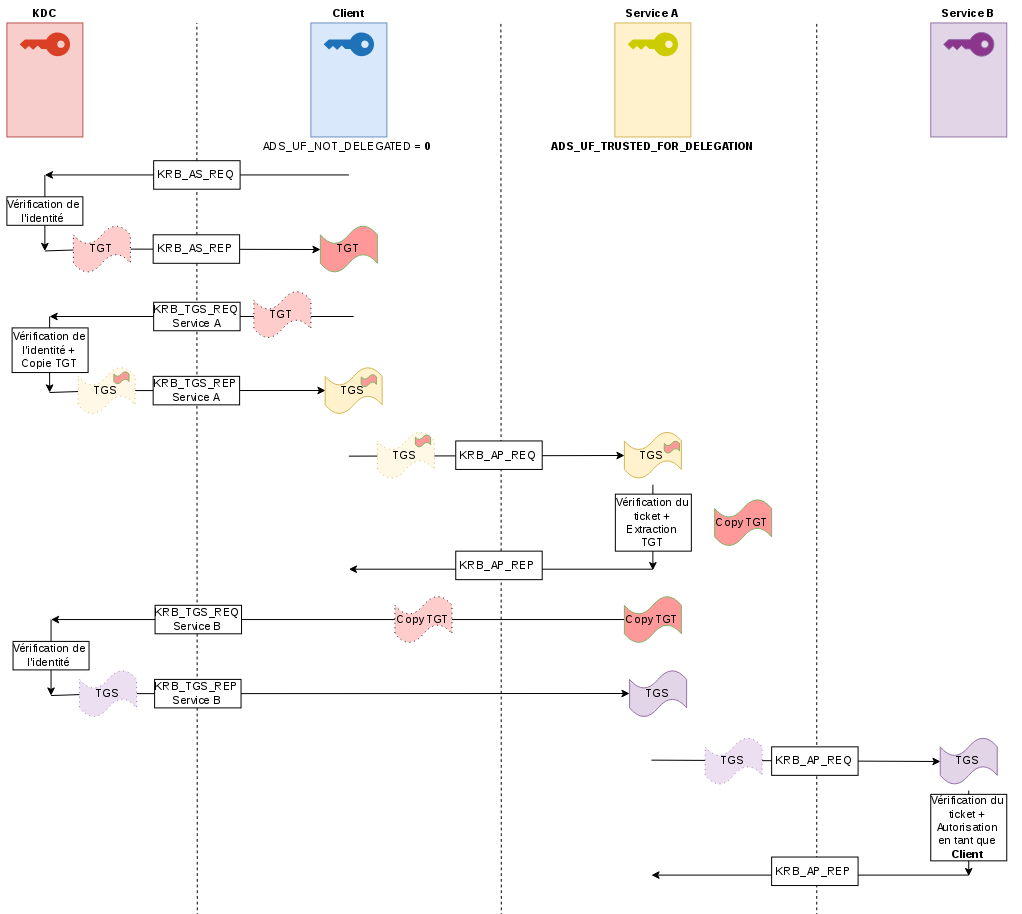
\includegraphics[width=\linewidth]{network/kerberos/images/unconstrained_delegation_detailed.png}
  \caption{unconstrained delegation detailed}
  \label{fig:unconstrained_delegation_detailed}
\end{figure}

The service will be able to decrypt the content of the TGS, verify the user’s identity by decrypting the authenticator, but above all it will be able to retrieve the copy of the TGT and the associated session key, in order to pretend to be the user at the Domain Controller.

{\bf The TGT and the session key are stored in LSASS}


\subsection{Service for User (S4U)}
\href{https://learn.microsoft.com/en-us/openspecs/windows_protocols/ms-sfu/3bff5864-8135-400e-bdd9-33b552051d94}{[MS-SFU]: Kerberos Protocol Extensions: Service for User and Constrained Delegation Protocol}

These protocol extension allow the support of constrained delegation. In essence, constrained delegation is a way to limit exactly what services a particular machine/account can access while impersonating other users.

There are two different Service for User (S4U) extensions:
\begin{itemize}
    \item {\bf S4U2proxy} enables a service to obtain a service ticket on behalf of the user to a second, back end service. 
    \item {\bf S4U2self}: Allows a service to obtain a Kerberos service ticket to itself on behalf of a user. This enables the service to obtain the user's authorization data that is then used in authorization decisions in the local service.
\end{itemize}



\subsubsection{Service for User to Proxy (S4U2proxy)}
\begin{figure}[!ht]
    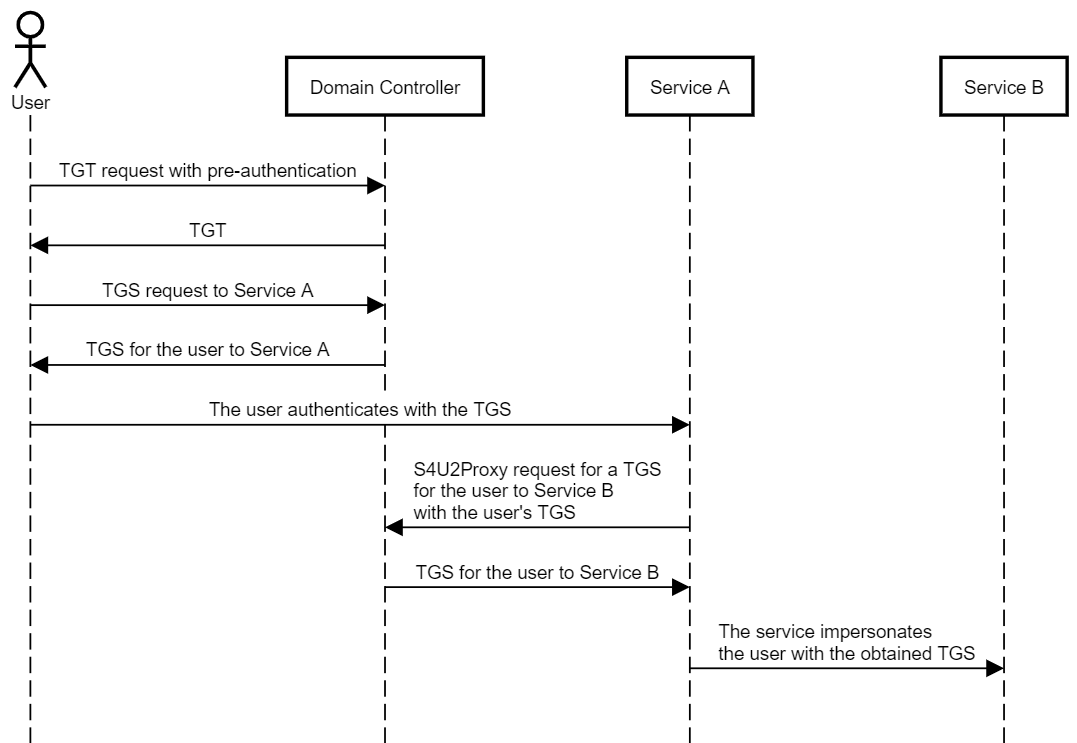
\includegraphics[width=\linewidth]{network/kerberos/images/S4U2Proxy.png}
    \caption{S4U2proxy}
    \label{fig:S4U2proxy}
\end{figure}

The user sends a TGS to access the service (“Service A”), and if the service is allowed to delegate to another pre-defined service (“Service B”), then Service A can present to the authentication service the TGS that the user provided and obtain a TGS for the user to Service B. Note that the TGS provided in the S4U2Proxy request must have the \verb+FORWARDABLE+ flag set. {\bf The \verb+FORWARDABLE+ flag is never set for accounts with \verb+USER_NOT_DELEGATED+ attribute is set to true or for members of the Protected Users group}. 

To tell the Domain Controller it wants to authenticate on behalf of someone else, two attributes will be defined in the \verb+KRB_TGS_REQ+ ticket request:
\begin{itemize}
    \item 
    The field \verb+additional-tickets+,must contain the user’s TGS (given that the \verb+NOT_DELEGATED+ flag is not set for the requesting user. If that was the case, the user’s TGS would not be forwardable, and the Domain Controller would not accept it in the rest of the process)
    \item 
    The \verb+cname-in-addl-tkt+ flag, which should be set to indicate to the Domain Controller that it should not use the server information, but the ticket information in additional-tickets.
\end{itemize}

If the targeted \verb+SPN+ is present in the \verb+msDS-AllowedToDelegateTo+ (or \verb+msDS-AllowedToActOnBehalfOfOtherIdentity+ in case of RBCD) then the Domain Controller sends back a valid \verb+TGS+, with the name of the user, for the requested service.

\subsubsection{Service for User to Self (S4U2self)}
Used to allow protocol transition. It allows a service to request a special forwardable service ticket to itself on behalf of a particular user.

\begin{figure}[!ht]
    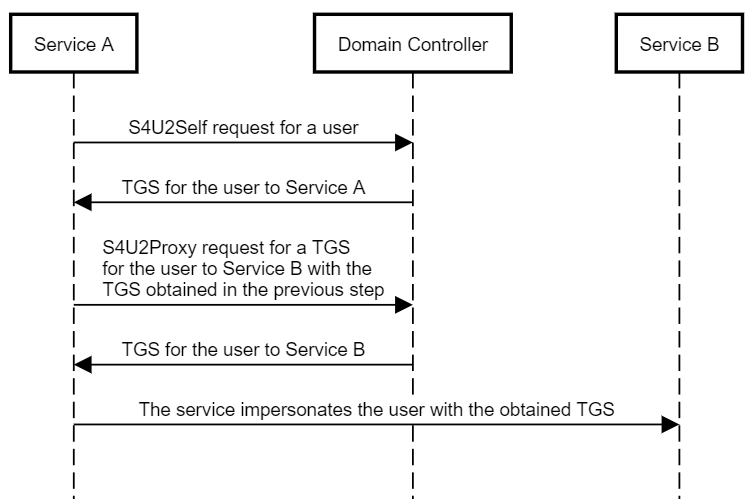
\includegraphics[width=\linewidth]{network/kerberos/images/S4U2Self.png}
    \caption{S4U2proxy}
    \label{fig:S4U2proxy}
\end{figure}

S4U2Proxy requires the service to present a TGS for the user to itself before the authentication service produces a TGS for the user to another service. It is often referred to as the “additional ticket”, but I like referring to it as “evidence” that the user has indeed authenticated to the service invoking S4U2Proxy. However, sometimes users authenticate to services via other protocols, such as NTLM or even form-based authentication, and so they do not send a TGS to the service. In such cases, a service can invoke S4U2Self to ask the authentication service to produce a TGS for arbitrary users to itself, which can then be used as “evidence” when invoking S4U2Proxy. To do this, it makes a classic \verb+TGS+ request (\verb+KRB_TGS_REQ+) except that instead of putting his own name in the \verb+PA-FOR-USER+ block (present in the pre-authentication part), it puts the name of a user it chooses.

This feature allows impersonating users out of thin air, and it is only possible when the \verb+TrustedToAuthForDelegation+ flag is set for the service account that invokes S4U2Self.


\subsection{Links}

\begin{itemize}
    \item \href{https://learn.microsoft.com/en-us/openspecs/windows_protocols/ms-sfu/3bff5864-8135-400e-bdd9-33b552051d94}{[MS-SFU]: Kerberos Protocol Extensions: Service for User and Constrained Delegation Protocol}
    \item \href{https://www.sstic.org/media/SSTIC2014/SSTIC-actes/secrets_dauthentification_pisode_ii__kerberos_cont/SSTIC2014-Article-secrets_dauthentification_pisode_ii__kerberos_contre-attaque-bordes_2.pdf}{Secrets d’authentification épisode II Kerberos contre-attaque - Aurélien Bordes}
    \item \href{https://blog.harmj0y.net/activedirectory/s4u2pwnage/}{S4U2Pwnage - Harmj0y}
    \item \href{https://shenaniganslabs.io/2019/01/28/Wagging-the-Dog.html}{Wagging the dog - Edla Shamir}
    \item 
        \url{https://book.hacktricks.xyz/windows-hardening/active-directory-methodology/constrained-delegation}
    \item 
        \url{https://www.secureauth.com/blog/kerberos-delegation-spns-and-more/}
\end{itemize}